%$$
%
\includegraphics[width=15cm]{GRAPHICS/PGL42_wedge_detached}
%$$
% file: PGL_6_2_sims_0.tex
% created by Orbiter tikz interface
% creation date: Sat Nov 13 14:23:37 +03 2021
% DeviceCoordinates 0 0 1000000 1000000
% UserCoordinates 0 0 10000 10000
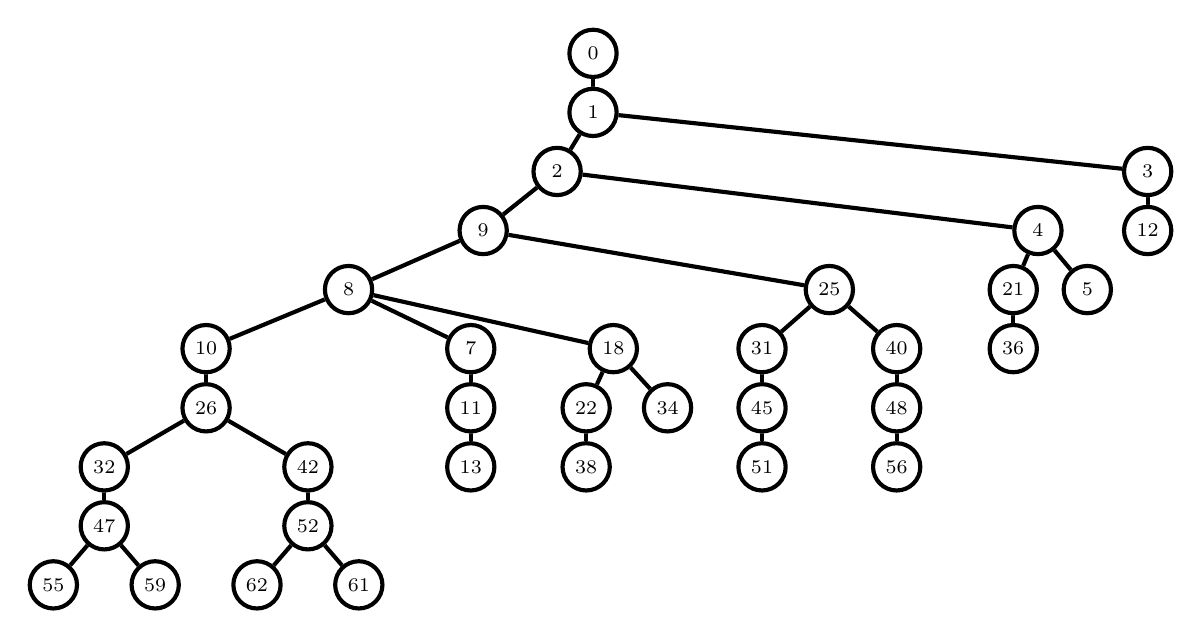
\begin{tikzpicture}[scale=0.45,line width = 1.5pt]
\draw [] (16.6667,32.5) -- (16.6667,30.8333);
\draw [] (16.6667,30.8333) -- (15.6533,29.1667);
\draw [] (16.6667,30.8333) -- (32.32,29.1667);
\draw [] (15.6533,29.1667) -- (13.5667,27.5);
\draw [] (15.6533,29.1667) -- (29.2233,27.5);
\draw [] (32.32,29.1667) -- (32.32,27.5);
\draw [] (13.5667,27.5) -- (9.76667,25.8333);
\draw [] (13.5667,27.5) -- (23.3367,25.8333);
\draw [] (29.2233,27.5) -- (28.5267,25.8333);
\draw [] (29.2233,27.5) -- (30.6167,25.8333);
\draw [] (9.76667,25.8333) -- (5.74667,24.1667);
\draw [] (9.76667,25.8333) -- (13.2167,24.1667);
\draw [] (9.76667,25.8333) -- (17.24,24.1667);
\draw [] (23.3367,25.8333) -- (21.4367,24.1667);
\draw [] (23.3367,25.8333) -- (25.2367,24.1667);
\draw [] (28.5267,25.8333) -- (28.5267,24.1667);
\draw [] (5.74667,24.1667) -- (5.74667,22.4967);
\draw [] (13.2167,24.1667) -- (13.2167,22.4967);
\draw [] (17.24,24.1667) -- (16.4733,22.4967);
\draw [] (17.24,24.1667) -- (18.77,22.4967);
\draw [] (21.4367,24.1667) -- (21.4367,22.4967);
\draw [] (25.2367,24.1667) -- (25.2367,22.4967);
\draw [] (5.74667,22.4967) -- (2.87333,20.83);
\draw [] (5.74667,22.4967) -- (8.62,20.83);
\draw [] (13.2167,22.4967) -- (13.2167,20.83);
\draw [] (16.4733,22.4967) -- (16.4733,20.83);
\draw [] (21.4367,22.4967) -- (21.4367,20.83);
\draw [] (25.2367,22.4967) -- (25.2367,20.83);
\draw [] (2.87333,20.83) -- (2.87333,19.1667);
\draw [] (8.62,20.83) -- (8.62,19.1667);
\draw [] (2.87333,19.1667) -- (1.43667,17.5);
\draw [] (2.87333,19.1667) -- (4.31,17.5);
\draw [] (8.62,19.1667) -- (7.18333,17.5);
\draw [] (8.62,19.1667) -- (10.0567,17.5);
\filldraw[color=white] (16.6667,32.5) circle [radius = 0.666667cm];
\draw (16.6667,32.5) circle [radius = 0.666667cm];
\draw (16.6667,32.5) node{{\scriptsize 0}};
\filldraw[color=white] (16.6667,30.8333) circle [radius = 0.666667cm];
\draw (16.6667,30.8333) circle [radius = 0.666667cm];
\draw (16.6667,30.8333) node{{\scriptsize 1}};
\filldraw[color=white] (15.6533,29.1667) circle [radius = 0.666667cm];
\draw (15.6533,29.1667) circle [radius = 0.666667cm];
\draw (15.6533,29.1667) node{{\scriptsize 2}};
\filldraw[color=white] (32.32,29.1667) circle [radius = 0.666667cm];
\draw (32.32,29.1667) circle [radius = 0.666667cm];
\draw (32.32,29.1667) node{{\scriptsize 3}};
\filldraw[color=white] (13.5667,27.5) circle [radius = 0.666667cm];
\draw (13.5667,27.5) circle [radius = 0.666667cm];
\draw (13.5667,27.5) node{{\scriptsize 9}};
\filldraw[color=white] (29.2233,27.5) circle [radius = 0.666667cm];
\draw (29.2233,27.5) circle [radius = 0.666667cm];
\draw (29.2233,27.5) node{{\scriptsize 4}};
\filldraw[color=white] (32.32,27.5) circle [radius = 0.666667cm];
\draw (32.32,27.5) circle [radius = 0.666667cm];
\draw (32.32,27.5) node{{\scriptsize 12}};
\filldraw[color=white] (9.76667,25.8333) circle [radius = 0.666667cm];
\draw (9.76667,25.8333) circle [radius = 0.666667cm];
\draw (9.76667,25.8333) node{{\scriptsize 8}};
\filldraw[color=white] (23.3367,25.8333) circle [radius = 0.666667cm];
\draw (23.3367,25.8333) circle [radius = 0.666667cm];
\draw (23.3367,25.8333) node{{\scriptsize 25}};
\filldraw[color=white] (28.5267,25.8333) circle [radius = 0.666667cm];
\draw (28.5267,25.8333) circle [radius = 0.666667cm];
\draw (28.5267,25.8333) node{{\scriptsize 21}};
\filldraw[color=white] (30.6167,25.8333) circle [radius = 0.666667cm];
\draw (30.6167,25.8333) circle [radius = 0.666667cm];
\draw (30.6167,25.8333) node{{\scriptsize 5}};
\filldraw[color=white] (5.74667,24.1667) circle [radius = 0.666667cm];
\draw (5.74667,24.1667) circle [radius = 0.666667cm];
\draw (5.74667,24.1667) node{{\scriptsize 10}};
\filldraw[color=white] (13.2167,24.1667) circle [radius = 0.666667cm];
\draw (13.2167,24.1667) circle [radius = 0.666667cm];
\draw (13.2167,24.1667) node{{\scriptsize 7}};
\filldraw[color=white] (17.24,24.1667) circle [radius = 0.666667cm];
\draw (17.24,24.1667) circle [radius = 0.666667cm];
\draw (17.24,24.1667) node{{\scriptsize 18}};
\filldraw[color=white] (21.4367,24.1667) circle [radius = 0.666667cm];
\draw (21.4367,24.1667) circle [radius = 0.666667cm];
\draw (21.4367,24.1667) node{{\scriptsize 31}};
\filldraw[color=white] (25.2367,24.1667) circle [radius = 0.666667cm];
\draw (25.2367,24.1667) circle [radius = 0.666667cm];
\draw (25.2367,24.1667) node{{\scriptsize 40}};
\filldraw[color=white] (28.5267,24.1667) circle [radius = 0.666667cm];
\draw (28.5267,24.1667) circle [radius = 0.666667cm];
\draw (28.5267,24.1667) node{{\scriptsize 36}};
\filldraw[color=white] (5.74667,22.4967) circle [radius = 0.666667cm];
\draw (5.74667,22.4967) circle [radius = 0.666667cm];
\draw (5.74667,22.4967) node{{\scriptsize 26}};
\filldraw[color=white] (13.2167,22.4967) circle [radius = 0.666667cm];
\draw (13.2167,22.4967) circle [radius = 0.666667cm];
\draw (13.2167,22.4967) node{{\scriptsize 11}};
\filldraw[color=white] (16.4733,22.4967) circle [radius = 0.666667cm];
\draw (16.4733,22.4967) circle [radius = 0.666667cm];
\draw (16.4733,22.4967) node{{\scriptsize 22}};
\filldraw[color=white] (18.77,22.4967) circle [radius = 0.666667cm];
\draw (18.77,22.4967) circle [radius = 0.666667cm];
\draw (18.77,22.4967) node{{\scriptsize 34}};
\filldraw[color=white] (21.4367,22.4967) circle [radius = 0.666667cm];
\draw (21.4367,22.4967) circle [radius = 0.666667cm];
\draw (21.4367,22.4967) node{{\scriptsize 45}};
\filldraw[color=white] (25.2367,22.4967) circle [radius = 0.666667cm];
\draw (25.2367,22.4967) circle [radius = 0.666667cm];
\draw (25.2367,22.4967) node{{\scriptsize 48}};
\filldraw[color=white] (2.87333,20.83) circle [radius = 0.666667cm];
\draw (2.87333,20.83) circle [radius = 0.666667cm];
\draw (2.87333,20.83) node{{\scriptsize 32}};
\filldraw[color=white] (8.62,20.83) circle [radius = 0.666667cm];
\draw (8.62,20.83) circle [radius = 0.666667cm];
\draw (8.62,20.83) node{{\scriptsize 42}};
\filldraw[color=white] (13.2167,20.83) circle [radius = 0.666667cm];
\draw (13.2167,20.83) circle [radius = 0.666667cm];
\draw (13.2167,20.83) node{{\scriptsize 13}};
\filldraw[color=white] (16.4733,20.83) circle [radius = 0.666667cm];
\draw (16.4733,20.83) circle [radius = 0.666667cm];
\draw (16.4733,20.83) node{{\scriptsize 38}};
\filldraw[color=white] (21.4367,20.83) circle [radius = 0.666667cm];
\draw (21.4367,20.83) circle [radius = 0.666667cm];
\draw (21.4367,20.83) node{{\scriptsize 51}};
\filldraw[color=white] (25.2367,20.83) circle [radius = 0.666667cm];
\draw (25.2367,20.83) circle [radius = 0.666667cm];
\draw (25.2367,20.83) node{{\scriptsize 56}};
\filldraw[color=white] (2.87333,19.1667) circle [radius = 0.666667cm];
\draw (2.87333,19.1667) circle [radius = 0.666667cm];
\draw (2.87333,19.1667) node{{\scriptsize 47}};
\filldraw[color=white] (8.62,19.1667) circle [radius = 0.666667cm];
\draw (8.62,19.1667) circle [radius = 0.666667cm];
\draw (8.62,19.1667) node{{\scriptsize 52}};
\filldraw[color=white] (1.43667,17.5) circle [radius = 0.666667cm];
\draw (1.43667,17.5) circle [radius = 0.666667cm];
\draw (1.43667,17.5) node{{\scriptsize 55}};
\filldraw[color=white] (4.31,17.5) circle [radius = 0.666667cm];
\draw (4.31,17.5) circle [radius = 0.666667cm];
\draw (4.31,17.5) node{{\scriptsize 59}};
\filldraw[color=white] (7.18333,17.5) circle [radius = 0.666667cm];
\draw (7.18333,17.5) circle [radius = 0.666667cm];
\draw (7.18333,17.5) node{{\scriptsize 62}};
\filldraw[color=white] (10.0567,17.5) circle [radius = 0.666667cm];
\draw (10.0567,17.5) circle [radius = 0.666667cm];
\draw (10.0567,17.5) node{{\scriptsize 61}};
\end{tikzpicture}
